
\subsection{Allocation Size for Small and Medium Pages}

Since small and medium pages only allow the user to allocate objects in certain size ranges, we can use this to our advantage to store metadata about the allocator in a more efficient way. Small pages allow objects sizes in the range [16B, 256KB] and medium pages (256KB, 4MB]. We note that the allowed sizes in the medium range is a factor of 16KB larger than the small range. This allows us to limit the allocator to the size range of small page, with an additional multiplication factor of 1 for small pages and 16KB for medium pages.

With the now limited allocation size range for small pages in mind, we are able to limit the number of free-lists we need and in turn the bits used in the bitmaps. We need 14 first-levels to be able to index every power of two inside the small page range, with a lower-bound of $2^4 =$ 16B and an upper-bound of $2^{17} =$ 128KB. It would be preferable to be able to store all bitmap information in a single 64-bit word for performance reasons, both in terms of cache efficiency and usage of efficient bit instructions. To stay inside the 64-bit limit we must choose the number of second-levels accordingly. For efficiency reasons, the number of second levels should be a power of two~\cite{tlsf}, and the only value this leaves us is 4, which requires $14 * 4 =$ 56 bits.

Combining the insight of the number of required first-levels, desire to use a single 64-bit bitmap and the number of second-levels, we can construct a new bitmap representation, as shown in Figure~\ref{fig:bitmap_flattening}. The new bitmap disregards the first-level bitmap entirely since the new bitmap can be indexed directly using the formula: $I = FL * 4 + SL$, where $FL$ is the first-level index and $SL$ the second-level index. Additionally, the lowest size classes have been placed at the least significant bits of the bitmap to make searching for the next non-empty free-list efficient using the find-first-set bit instruction.

\begin{figure}[H]
    \centering
    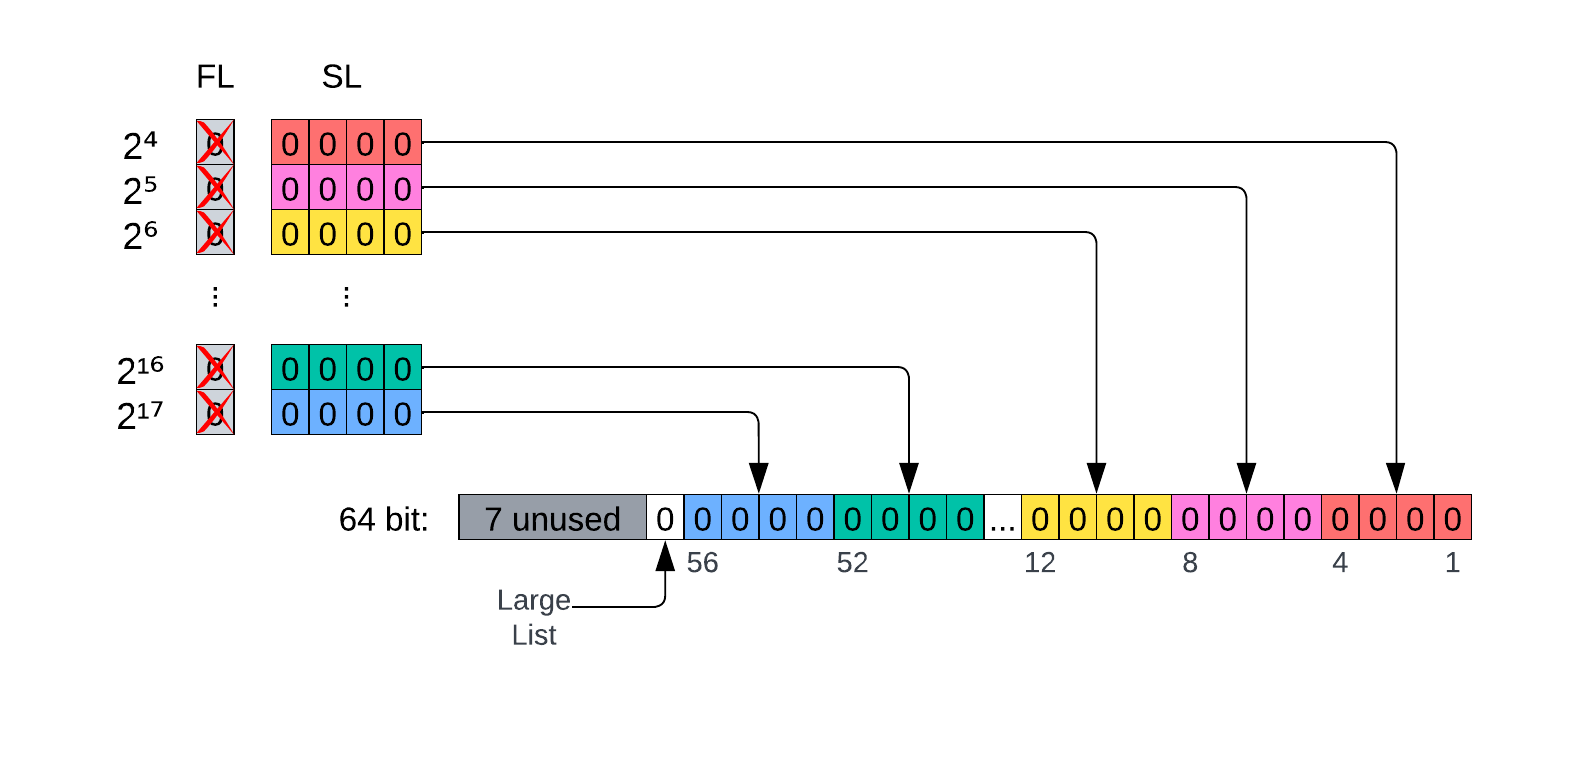
\includegraphics[width=1\textwidth]{figures/bitmap_flattening.png}
    \caption{Flattening of the 2D-matrix reprsentation of TLSF bitmaps into a single 64-bit value. The first-level bitmap is disregarded in favor of indexing the new flattened bitmap using the first-level value instead. The number of first-levels are 14, indicated by bits of the same color belonging to the same first-level. The number of second-levels are 4, as indicated by the same number of colored bits.}
    \label{fig:bitmap_flattening}
\end{figure}

The relationship between the bitmap and the free-lists is illustrated in Figure~\ref{fig:bitmap_relationship}, closely adhering to the original TLSF design. However, the adaptation now figures out what free-list to look at from the new 64-bit bitmap.

\begin{figure}[H]
    \centering
    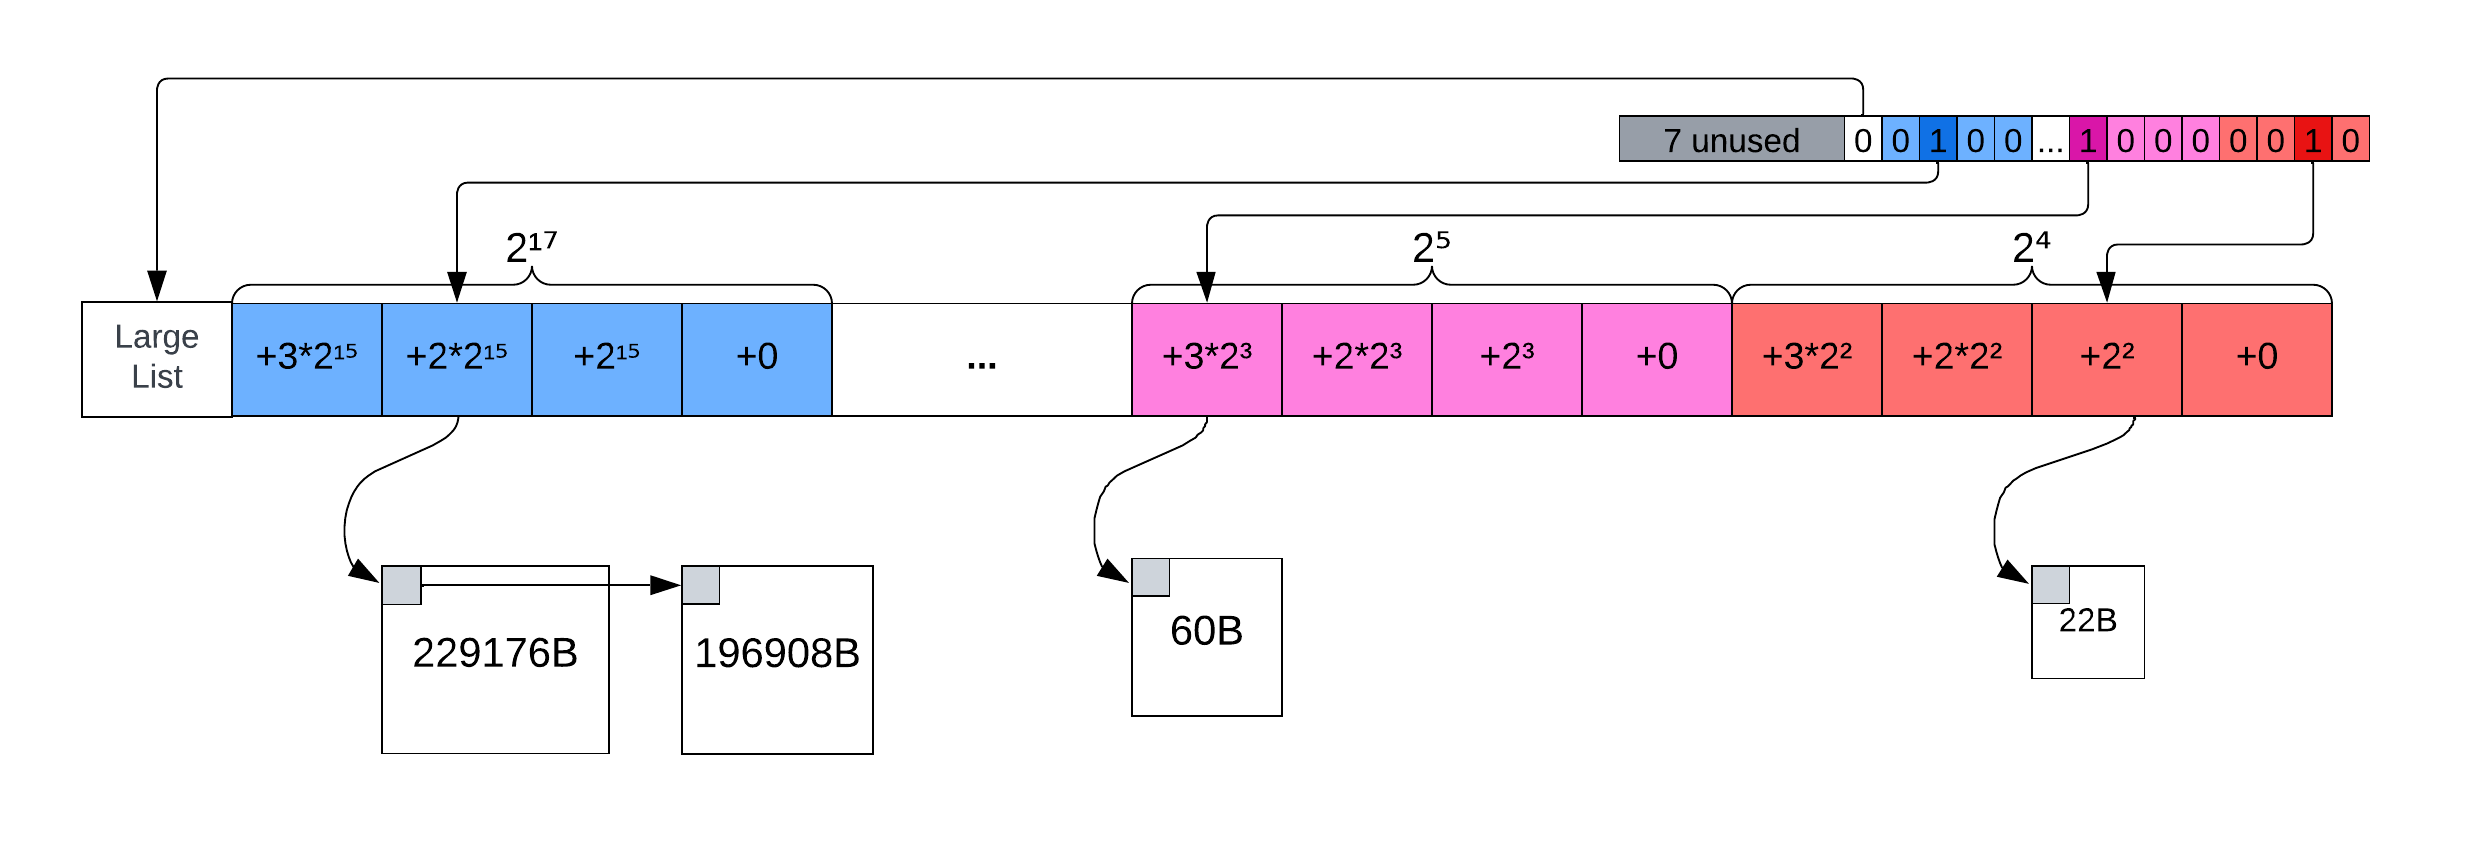
\includegraphics[width=1\textwidth]{figures/bitmap_relationship.png}
    \caption{Relationship between the new bitmap representation and accessing the corresponding free-lists.}
    \label{fig:bitmap_relationship}
\end{figure}

% TODO: Detta borde flyttas till discussion.
% A drawback of dividing the memory into only four second-levels per fist-level is that there is less chance that a block is closer to the size that we want to allocate. This could potentially lead to higher fragmentation, as there are fewer size classes of blocks available. However, this is generally not a problem...

% TODO: Cite TLSF paper.
% Benefits: Reduced memory overhead, cache efficiency, Simplified indexing (and Atomic operations??)
% Drawbacks: Reduce number of second-level partitions to 4, instead of more, which could have an impact on internal fragmentation.

%%% Local Variables:
%%% mode: latex
%%% TeX-master: "main"
%%% End:
